\section{Search With Clojure}
	Clojure's excellent \gls{jvm} interoperability permits the use of countless third-party libraries.  The most extensively used was Lucene.
	
	\subsection{Full-Text Search Using Lucene}
		\textcquote{luc-home}{Apache Lucene\texttrademark\ is a high-performance, full-featured text search engine library written entirely in Java.}
	
	\subsection{Indexing Relational Database}
		The process of indexing a relational database is a multi-step one.  It begins with the declaration of the database connection information, the path to the index, and the schema definition.
		
		In our implementation, this information is specified by a record that adheres to the protocol in \vref{clj:iconfig}.  The record which defines the Mycampus dataset uses SQLite for its database engine, so it accepts two strings; one specifies the path to the database file, while the other specifies the path to the index.
		
		\begin{figure}
			\begin{singlespaced}
				\cljcode[firstline=16,firstnumber=16,lastline=19]{../../src/clj/molly/conf/config.clj}
			\end{singlespaced}
			
			\caption{\texttt{IConfig} protocol all configurations must adhere to}
			\label{clj:iconfig}
		\end{figure}
		
		The first component, \texttt{connection}, returns a \gls{jdbc}-compatible object.  The second component, \texttt{schema}, returns a list of \texttt{EntitySchema} records.  The \texttt{EntitySchema} record is defined in \vref{sec:entity-schema}.  The final component, \texttt{index}, specifies the path to the index.
		
		\subsubsection{Schema Graph Definition}
		\label{sec:entity-schema}
			The schema graph is defined using Korma, which \textcquote{clj-korma}{is a \gls{dsl} for Clojure}.  Each schema component, whether an entity or entity group, is defined by \texttt{EntitySchema} records.  Each record accepts a map which specifies how each class of document should be indexed and identified.  The keys of this map are given in \vref{tbl:entity-schema-keys}.
			
			\begin{table}
				\centering
				
				\begin{tabular}{lp{9cm}l}
					\toprule
					Key & Description & Type(s) \\
					\midrule
					\texttt{:T} & Entity (\texttt{:entity}) or entity group (\texttt{:entity}) & Symbol \\
					\texttt{:C} & Table name for entities, brief description for entity groups & Symbol or String \\
					\texttt{:sql} & \Gls{sql} query used to construct the entity or entity schema & Expression \\
					\texttt{:ID} & Attribute or attributes that comprise the key (\vref{def:keys}) & Symbol or list of symbols \\
					\texttt{:attrs} & List of attributes to analyze to fields & List of symbols \\
					\texttt{:values} & List of attributes to index as values, must be subset of \texttt{:attrs} & List of symbols \\
					\bottomrule
				\end{tabular}
				
				\caption{Keys expected by \texttt{EntitySchema} records}
				\label{tbl:entity-schema-keys}
			\end{table}
			
			The \texttt{EntitySchema} records contain not only the information required to construct them, but also the required behaviour.  Every record, given the database and index connections, is capable of retrieving the set of all named tuples it represents in the database.  It iterates through every tuple and constructs a document for each tuple, as well as any value documents, if applicable.
			
		\subsubsection{Indexing Process}
			With the database, index, and schema graph defined, the system is able to transform the data from the relational model into the document model.  The first step is to open the database for reading and the index for writing.  This paths to the database and index are given by the \texttt{.properties} file.
			
			The second step is to read in the configuration file which describes the schema graph.  The schema graph is given as \texttt{EntitySchema} records.  These records contain the \gls{sql} required to retrieve the named tuples from the database, as well as other information required to transform each named tuple into a document.
			
			The indexing process iterates over every \texttt{EntitySchema} record, calling the \texttt{crawl} function on each one.  The \texttt{crawl} function uses the configuration map attached to the \texttt{EntitySchema} record to construct itself.uf, which in turn executes a \gls{sql} query using \texttt{execute-query} (defined by the \texttt{Database} protocol).  For every named tuple, a function (provided by the \texttt{EntitySchema} record) is executed on it.
			
			%The first half of the indexing process is shown in \vref{fig:indexing-process-first-step}.
			
			%\begin{figure}
			%	\centering
			%	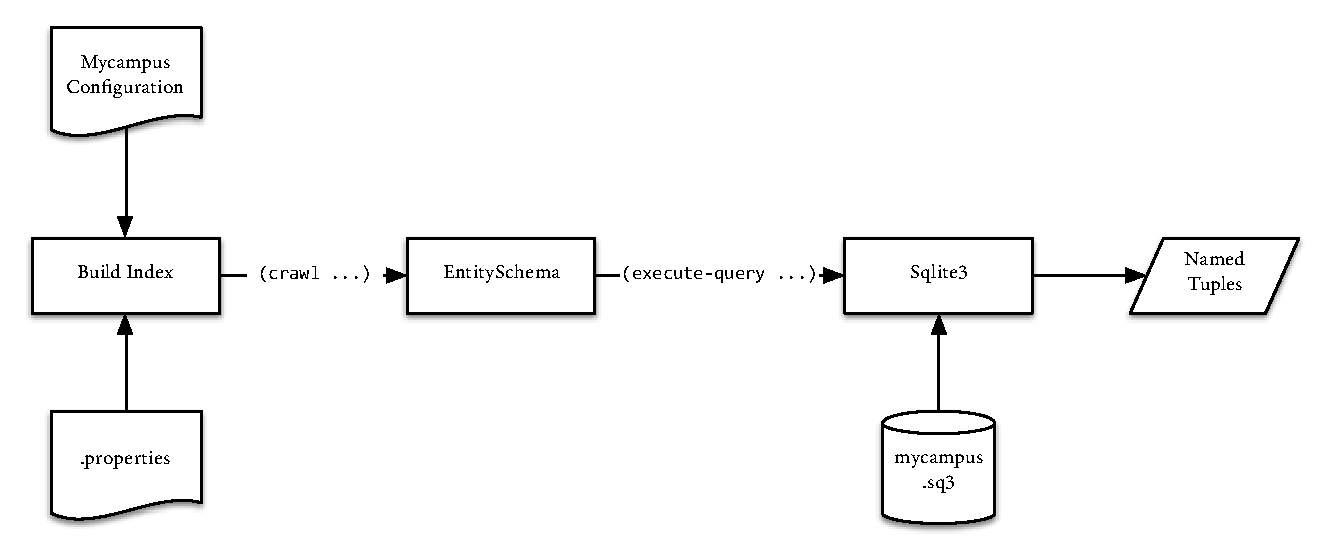
\includegraphics[scale=0.7]{figures/diagrams/indexing-process}
			%	
			%	\caption{First part of indexing process demonstrating how named tuples are generated}
			%	\label{fig:indexing-process-first-step}
			%\end{figure}

	\subsection{Indexing of relational objects (5 days, week 5)}
		\begin{itemize}
			\item Schema definition
			\item Crawling using SQL
			\item Indexing using relational objects
			\item Fuzzy indexing of values (typed by classes)
		\end{itemize}

	\subsection{Keyword Search in document space (5 days, week 6)}
		\begin{itemize}
			\item Disambiguate keywords using fuzzy search (suggestion, overloaded terms)
			\item Flexibility keyword search for documents
			\item Translate search result back to relational space
		\end{itemize}

	\subsection{Graph Search in document space (5 days, week 7)}
		\begin{itemize}
			\item Why we need graph search
			\item Search in document graph using graph search algorithms with functional implementations: (Ford Fulkerson, BFS)
			\item Speed up using concurrency
			\item Clojure specific optimization: ref + atom
		\end{itemize}